\chapter{引言}
\label{cha:intro}

\section{研究背景和研究意义}

\footnotetext[1]{Hadoop.~http://hadoop.apache.org/.}
\footnotetext[2]{Spark.~http://spark.apache.org/.}
\footnotetext[3]{Flume.~http://flume.apache.org/.}
\footnotetext[4]{Storm.~http://storm-project.net/.}
\footnotetext[5]{Ceph.~http://ceph.com.}
云计算技术是 IT 产业界的一场技术革命, 已经成为了 IT 行业发展的一个大方向。 
各国政府纷纷将云计算服务视为国家软件产业发展的新机遇。 
美国政府在IT政策和战略中也加入了云计算因素,美国国防信息系统部门 (DISA) 正在其数据中心内部搭建云环境\cite{fang-cloud}。
作为云计算的承载体-数据中心,近些年也收到了越来越多的关注。
事实上,从2010年起 , 全球数据中心的市场规模一年比一年庞大,
已经从2010年的20亿美元提高到了2015年的4.6亿美元,平均每年增长幅度达到了$14.3\%$\cite{wu-datacenter}。
所谓数据中心,就是一套由计算机及相关配套设备所组成的,
以储存、传递、展示、加工处理数据为主要目的的完善系统工程\cite{wu-datacenter}。
现在很多应用都部署在数据中心,为用户提供各种各样的服务,
例如,为用户提供计算服务的Hadoop \footnotemark[1]、Spark \footnotemark[2]、Flume \footnotemark[3]、Storm \footnotemark[4]等,为用户提供存储的ceph \footnotemark[5]等。
甚至,很多企业比如国外的facebook,youtube,国内的中国银行,中国电信等,都有自己的数据中心。
数据中心已经成为国内国外工业界和学术界关注的重心和研究热点。

在实际中,数据中心有成千上万台机器。
根据统计,截止2016年,
谷歌的数据中心中有多达45万台机器\cite{wei-dc}。
在数据中心的服务器中,部署着各种各样的应用,因为单个机器的
计算能力,容量等有限,而具有超高计算能力和超高存储能力的大型计算机的成本又太高,
因此,应用往往采取分布式的方法部署在集群中。
部署在集群中的应用数据流族,有共同的目标和共同的语义,
它们或是计算同一个目标,
或者是作为存储同一个巨型文件,
或者是为了达到同一个优化目标等。
各种各样的分布式应用部署在数据中心,
突出了数据中心作为信息服务载体的核心地位,
也同时给数据中心的建设提出了更加严峻的挑战。


数据中心网络(Data Center Networks,简称 DCNs)是指数据中心内部通过高速链路和交换机,路由器连接大量服务器的网络。
传统数据中心网络主要采用层次结构实现,
且承载的主要是客户机/服务器模式的应用。
多种应用同时在同一个数据中心内运行,每种应用一般运行在其特定的服务器/虚拟服务器集合上\cite{wei-dc}。
因为数据中心的应用常常分布式的部署在集群中,
而这些应用常常需要多个计算或者存储步骤才能得到预期的结果。
数据中心应用内部,应用之间往往进行频繁的通信,
数据中心网络,就是这些应用通信的桥梁。
作为数据中心中应用传输的媒介,随着数据中心规模的变大,
应用对数据中心网络提出了越来越高的要求,
网络性能已经逐渐成为数据中心发展的瓶颈。
在网络给数据中心提供的服务中,
应用获得的带宽和传输的延迟,是评价服务质量高低重要的因素。
应用的带宽和传输延迟常常对用户体验产生重要的影响。
根据facebook的报告\cite{Latency},应用的延迟每增加100毫秒,收入会减少1$\%$。


因此,越来越多的研究,集中在优化数据中心应用的带宽和延迟上。
互联网采用TCP作为传输协议。
直接在数据中心采用TCP会导致一系列问题:
首先,TCP采取滑动窗口机制进行控制,
当发生拥塞时,交换机会出现丢包,此时发送端的拥塞窗口会减半,从而发送端速率会减小。
滑动窗口减半会引发链路震荡大,从而链路利用率低。
没有拥塞时,发送端的拥塞窗口会不断增大,发送端速率不断增大,从而导致交换机缓冲区不断变大,引起较大的排队延迟。
此外,TCP是公平分配带宽的策略,然而对于数据中心的应用而言,不同的应用对延迟和带宽的需求是不同的。
应用如时钟同步,Memcached,Naiad等需要数据中心网络提供低延迟,
而hadoop等计算应用需要数据中心网络提供高带宽。
事实上,数据中心的资源总量是一定的,
采用TCP进行传输,不能有效的满足应用对延迟和带宽的需求,造成数据中心网络资源不能合理高效的使用。
当前,越来越多的应用部署在规模日益增大的数据中心集群中,
给数据中心网络带来了各种各样的问题和挑战,
如何合理的分配数据中心网络资源,
使得数据中心能够满足日益增加的网络需求,
是当前业界面临的一个重大挑战。


针对上述的问题,本文对数据中心的应用传输做优化,
从而应用可以提供更好的用户体验,
并可以充分合理的利用信道,提高资源利用率。
本文的工作重点是:一是从流级别进行传输优化,改进数据传输协议,
使应用可以根据网络拥塞状况和应用的期限等因子调整带宽。
从而使得不同需求的应用获得不同大小的带宽。
二是为数据中心任务分配优先级,采用集中式的方法,
使的网络资源的分配可以根据应用的优先级和网络拥塞进行动态调配。
从而可以提高用户体验,同时可以使的网络资源利用率高。
需要说明的是,本文提供的方法,不止用于数据中心网络,
也可以用于其他类似网络环境下。
\label{cha:LPD}
\begin{figure}[b]
\begin{center}
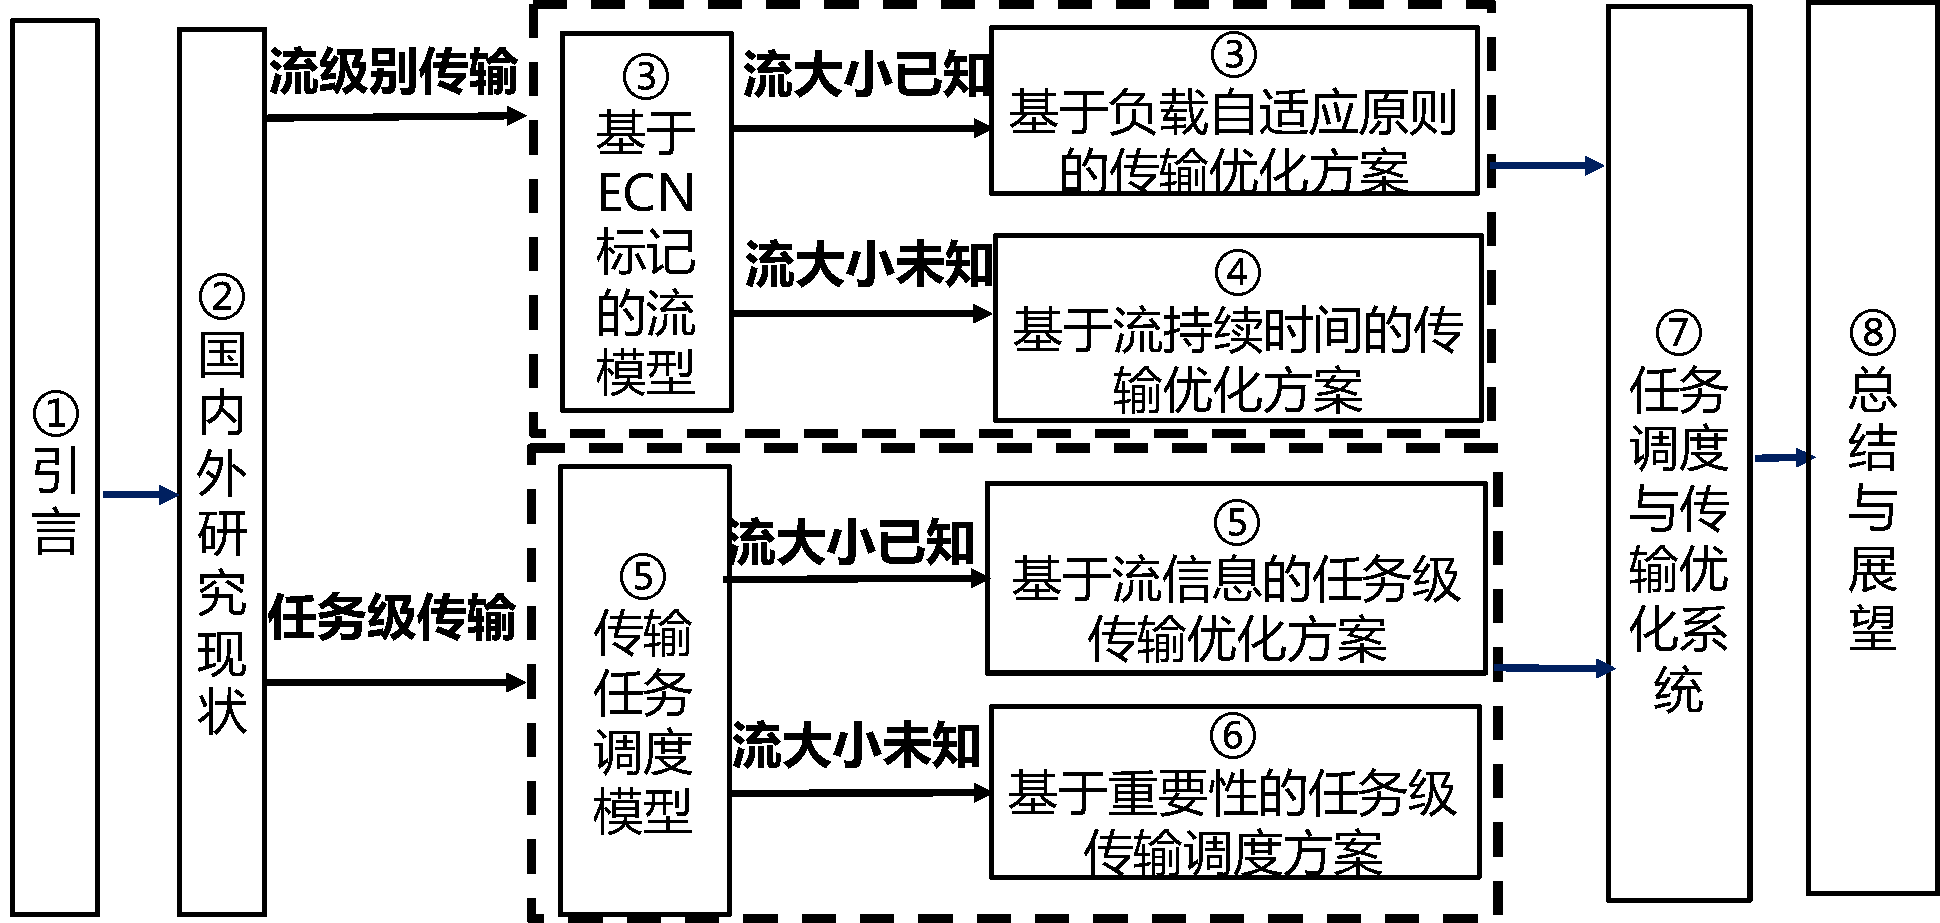
\includegraphics [width=0.9\columnwidth] {figures/structure.pdf}
\caption{论文结构}
\label{paper-structure-fig}
\end{center}
\end{figure}


\section{论文研究内容}
作者的博士论文主要包括以下几个方面:

\textbf{(1)~综述了国内外研究现状}

本文介绍数据中心应用传输方案的相关工作。
首先,从常见应用的通信模型和数据流量等方面对数据中心传输进行概述。
本文重点介绍4类通信模型:映射规约模型(Map-Reduce),数据流模型(Dataflow),
大型并行数据传输模型(Bulk Synchronous Parallel ),分区-聚合模型(partition-aggregate),并介绍了查询流,
背景流等流量特征和数据中心应用期限等特征。
因为传统的TCP协议,难以满足不同的应用对带宽和延迟的需求,
本文从流级别和任务级别对数据中心传输方案进行综述。
最后,本文总结数据中心传输方案存在的问题。

\textbf{(2)~研究了基于ECN标记的流传输模型}

本文介绍基于ECN标记的流模型。
首先,对基于ECN标记的流模型的场景进行介绍。
然后,介绍了基于ECN标记的流模型,
最后,根据基于ECN标记的流模型实例化DCTCP,
得到DCTCP流模型,
作为ECN标记的流模型的一个实例,
并使用ns-2和流模型进行比对。

\textbf{(3)~研究了基于负载自适应原则的传输优化方案 }

现在很多在线应用部署在数据中心,数据中心网络的性能和底层技术吸引了越来越多的研究者的兴趣。
为了达到更好的网络性能,
近期的研究从不同角度优化数据中心网络流量传输和调度,并且设计各种路由和传输方案。
特别是对于必须及时为用户服务的应用,数据流的传输应尽快的完成,有的必须在截止时间之前完成,
最近业界出现了一系列的考虑流传输期限的网络流量控制策略。
本文主张在设计数据流传输方案时,
应该遵循一个简单的原则:
拥有不同截止期限的流在其带宽分配和占用上应该被区分,
网络负载越重,数据流越被区分。
本文认为设计流量控制策略时应该遵循这个原则。
根据这个原则,本文并提出了一种简单的拥塞控制算法-正比负载差分
(Load Proportional Differentiation,简称LPD)作为其应用。
在不同的仿真环境和测试床上,针对不同的网络拓扑和负载情况下评估了LPD的性能。

\textbf{(4)~研究了基于流持续时间的传输优化方案}

数据中心现在正成为许多应用(如网络搜索和零售)的部署平台。
由于TCP不能满足应用程序对延迟和吞吐量的要求,因此提出了许多基于TCP的协议(例如,DCTCP,D$^2$TCP,L$^2$DCT)来对TCP进行补充。
其中,D$^2$TCP等协议将明确的截止时间纳入拥塞窗口调整过程,以保证流在截止时间之前完成。
L$^2$DCT等协议在计算拥塞窗口调整因子时考虑流量大小,保证短流量的吞吐量和延迟。
这两种方法在一定的场景下运行良好,但在两个方面存在一些不足。
首先,这两种方法只能减小流错失期限的百分比或者能够减小短流的延迟,但是不能够同时优化这两个目标。
其次,这些方法中的大多数都需要用户知道流的信息(例如截止时间,流量大小),这些信息对于一些应用来说,可能很难事先确切得知。
本文主张引入流持续时间进入拥塞窗口调整的过程中。
基于此,本文提出基于流持续时间速率控制(Flow Duration Rate Control,简称FDRC)机制。
本文发现,在不得知流具体信息的情况下,FDRC可以达到同时减少流错失期限的比例和减小流平均完成时间。
本文从理论上分析了FDRC的行为,并在ns-2和Iinux内核实现FDRC。

\textbf{(5)~研究了数据中心任务级传输优化模型}

本文对数据中心任务传输模型进行介绍,首先,本章从数据中心非阻塞模型, 
以及传输任务等对数据中心任务级传输的模型进行介绍。
随后介绍数据中心 任务调度问题的复杂度,最后,
引入任务的离线调度算法,并证明离线调度算法的近似度。

\textbf{(6)~研究了基于流信息的任务级传输优化方案 }

随着大数据应用的部署,越来越多的数据存储在大数据存储系统中。
大数据存储系统希望给用户提供安全,稳定,高效的文件存取服务。
纠删码存储系统已被诸如Google和Facebook等公司广泛使用,因为它使用纠错码来保证文件系统的可靠性。
在纠删码存储系统中,使用(n,k)MDS纠删码用于将文件分成n个块。
当用户想要访问文件时,文件系统可以选取n个块中的任何k个子集来重建文件。
在这种情况下,如何从n个数据块中选出k个数据集,如何高效的传输这k个数据块,成为一个重要的问题。

\textbf{(7)~基于重要性和网络拥塞的任务传输调度方案}

传统的网络资源管理机制主要是流级别或者包级别的。
最近,流组(coflow)作为一种新的并行应用数据传输通信的抽象模型而提出。
流组(coflow)对网络资源的应用级语义进行了有效的建模,因此可以通过将流组(coflow)作为网络资源分配或调度的基本元素来更好地实现一些高级优化目标,如减少应用程序的传输延迟等。
虽然有效的流组(coflow)调度方法已经被研究,
但是应用的重要性等因素并没有被考虑,如何根据应用的重要性和coflow的特性对应用进行调度是一个重要问题。

\textbf{(8)~设计并实现和评估了数据中心应用传输优化系统}

本文设计并实现了数据中心传输系统 FlyTransfer,
并介绍了 FlyTransfer 系统架构和系统的各个组件。
随后使用数据中心真实流量,从任务级别调度,流级别优化和系统开销等方面对系统进行性能评估。

\section{论文的主要贡献}
\textbf{(1)提出了基于负载自适应原则的传输优化方案}

本文主张在设计数据流传输方案时,
应该遵循一个简单的原则:
拥有不同截止期限的流在其带宽分配和占用上应该被区分开,
网络负载越重,数据流越被区分。
本文认为设计流量控制策略时应该遵循这个原则。
根据这个原则,本文提出了一种简单的拥塞控制算法-正比负载差分
(Load Proportional Differentiation,简称LPD)算法作为其应用。
本文在不同的拓扑和负载场景下评估LPD,并对LPD进行仿真和测试床评估。
与D$^2$TCP(最先进的基于期限的拥塞控制策略)相比,
使用LPD,错过最后期限的流比例减少25$\%$以上。
与Karuna相比,LPD平均有5$\%$的性能损失。
但是在拥塞严重的情况下,LPD的性能比Karuna高5$\%$ - 10$\%$。
事实上 “越拥塞,越区分”是一个通用的原则,它也可以用于其他目标的优化,比如优化流平均完成时间。
与基于窗口的协议L$^2$DCT相比,LPD可以将流平均完成时间减少30$\%$。
和最先进的流平均完成时间优化策略pFabric相比,LPD的性能比之差20$\%$。 

\textbf{(2)提出了基于流持续时间的传输优化方案}

在本文中,我们主张使引入流持续时间进入拥塞窗口调整的过程。
基于此,我们提出基于流持续时间速率控制机制(Flow Duration Rate Control,简称FDRC)。
本文发现,无需得知流信息的前提下,FDRC可以同时减少流错失期限的比例并且减小流平均完成时间。
本文从理论上分析了FDRC的性能,并在ns-2和Iinux内核实现FDRC。
实验表明,在几乎所有场景下,FDRC比D$^2$TCP和L$^2$DCT的性能都要好。
平均来说,FDRC比D$^2$TCP性能高30$\%$,比L$^2$DCT,性能提高大约10$\%$。



\textbf{(3)提出了基于流信息的任务级传输优化方案}

本文使用纠删码存储系统为例,进行最小化文件平均访问时间(File Access Time,简称FAT)的优化。
为了实现这一点,本文提出了最小负载优先的启发式算法做为纠删码存储系统数据源选取的策略。
并且从任务级别对传输系统进行优化。
在此基础上,本文设计并实现了D-Target,
一个集中调度器,对纠删码存储系统的传输进行调度。
最后,通过AT\&T的的存储系统数据验证D-Target的性能。
结果表明,
D-Target在FAT性能方面分别比TCP,Aalo,Barrat和pFabric分别提高了2.5$\times$,1.7$\times$,1.8$\times$。

\textbf{(4)提出了基于重要性和网络拥塞的任务传输调度方案}

本文提出加权流组完成时间(Weighted Coflow Completion Time,简称WCCT)最小化问题,
同时针对此问题,设计了不需要知道流大小就可以进行调度的在线算法-Yosemite。
Yosemite可以根据流组权重和网络拥塞程度进行流组调度。
然后,本文通过数据中心的真实流量对系统进行仿真评测。
实验结果结果显示,与最新的流组调度算法相比,
Yosemite可以使得平均WCCT减少超过$40\%$,
对于重要性在平均程度以上的流组,流组的平均完成时间减少超过$30\%$。
和最有效的流组调度方法相比,针对WCCT优化的性能大约提高了$30\%$,
对于重要性在平均以上的流组,平均完成时间减少大约$25\%\sim30\%$。


\section{论文的组织结构}
如图\ref{paper-structure-fig}所示,本文总共分为10章,其中第2章到第9章是论文的主体部分。
第1章,是论文的引言部分。
主体部分主要包括流级别的优化,任务级别的优化和应用传输系统的介绍。
其中,论文的第3章到第5章侧重流级别的传输优化。
第3章介绍的是基于 ECN 标记的流模型,
第4章介绍的是基于负载自适应原则的传输优化方案,
第5章介绍的是基于流持续时间的传输优化方案。
本文的第6到8章介绍的是任务级传输优化方法,
其中第6章介绍的是任务级别速率和延迟优化模型,
第7章介绍的是任务级的纠删码传输优化系统,
第8章介绍基于重要性和网络拥塞的任务传输优化。
第9章是论文的第三部分,主要介绍应用传输系统FlyTransfer以及其性能评测。
第10章是论文的总结部分,主要是对当前工作的总结和对未来工作的展望。


